\documentclass[12pt]{article}
\usepackage{parskip}
\usepackage{amsmath}
\usepackage{pdfpages}
\usepackage{listings}
\usepackage{color}
\usepackage[margin=.6in]{geometry}

\definecolor{dkgreen}{rgb}{0,0.6,0}
\definecolor{gray}{rgb}{0.5,0.5,0.5}
\definecolor{mauve}{rgb}{0.58,0,0.82}

\lstset{frame=tb,
  language=C++,
  aboveskip=3mm,
  belowskip=3mm,
  showstringspaces=false,
  columns=flexible,
  basicstyle={\small\ttfamily},
  numbers=none,
  numberstyle=\tiny\color{gray},
  keywordstyle=\color{blue},
  commentstyle=\color{dkgreen},
  stringstyle=\color{mauve},
  breaklines=true,
  breakatwhitespace=true,
  tabsize=3
}
\begin{document}
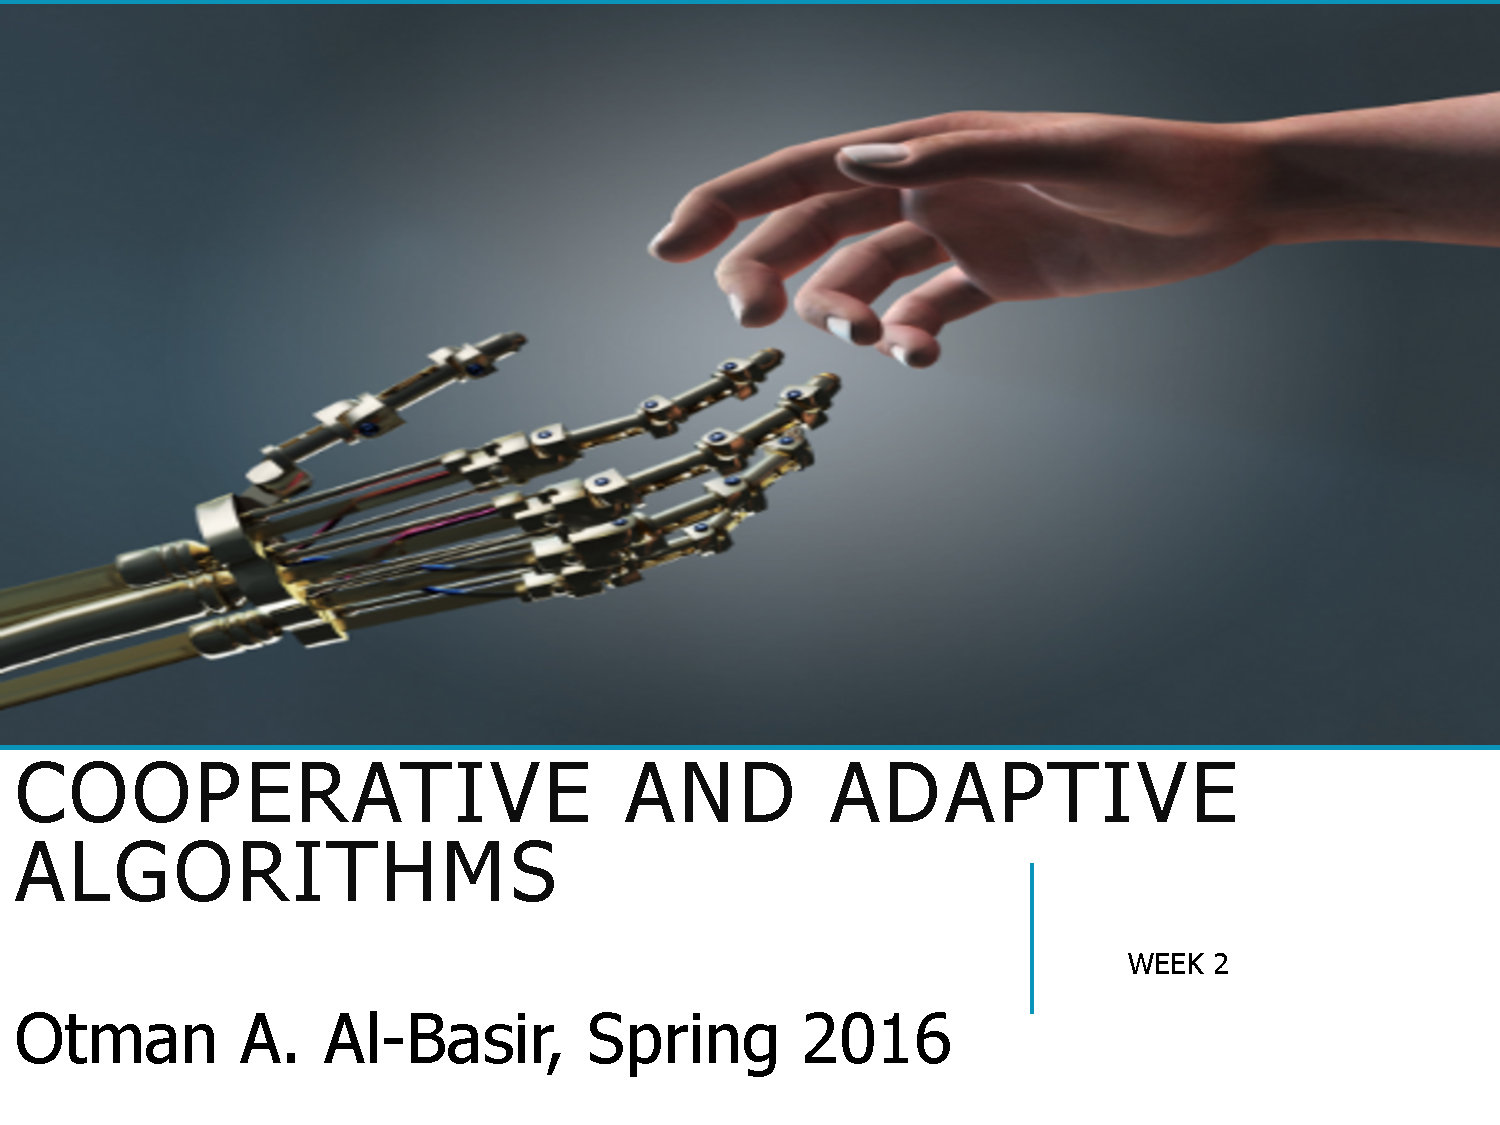
\includepdf[pages=1-2]{slides.pdf}
\includepdf[pages=3]{slides.pdf}
When we have a blind search (uninformed) we just compete against other strategies with nothing to do with the promise of the actions. 

\includepdf[pages=4-5]{slides.pdf}
\paragraph{Breadth First Search} % (fold)
\label{par:breadth_first_search}
We move sideways across a tree through an entire level before moving down. 
% paragraph breadth_first_search (end)

\includepdf[pages=11-13]{slides.pdf}
Bredth first search is not always the best, but we can sort shit while we build the tree to make it better. We start at S and sort nodes by their path cost which places a, b, and c. Then we add G who's cost is 11 (1+10). Then we add the remaining links to G (these numbers are given).t

\includepdf[pages=14-16]{slides.pdf}
Basically we investigate each layer as you would a bredth first serach, but you check the lowest cost first.

\includepdf[pages=17]{slides.pdf}
\includepdf[pages=26]{slides.pdf}
Depth first search also works pretty well. Mother fucker, you know how depth first search works.

\includepdf[pages=29]{slides.pdf}
\includepdf[pages=32]{slides.pdf}
We want to make sure that shit doesnt run indefinitly so we put a bound on how many layers you go down. 

\includepdf[pages=33]{slides.pdf}
To do this we first iterate down to a set depth. If you dont find up to the depth we begin again with a bounded depth first search 

\end{document}